\section{Il bilancio di esercizio}
\subsection{Il modello del bilancio: Archetipo economico-finanziario}

\begin{figure}[H]
    \centering
    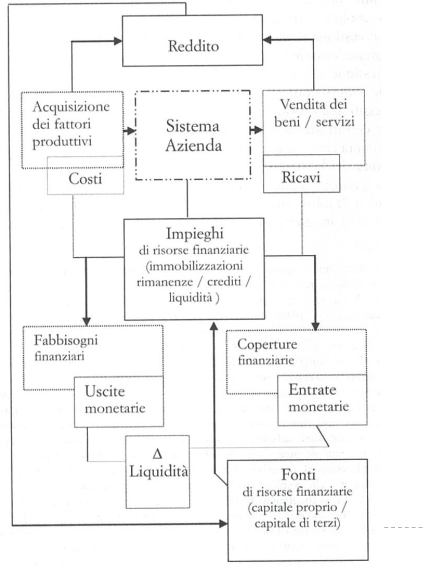
\includegraphics[width=0.4\linewidth]{2/img/Screenshot from 2022-07-09 16-49-15.png}
\end{figure}

\subsection{Il modello del bilancio: I prospetti numerici}


\begin{figure}[H]
    \centering
    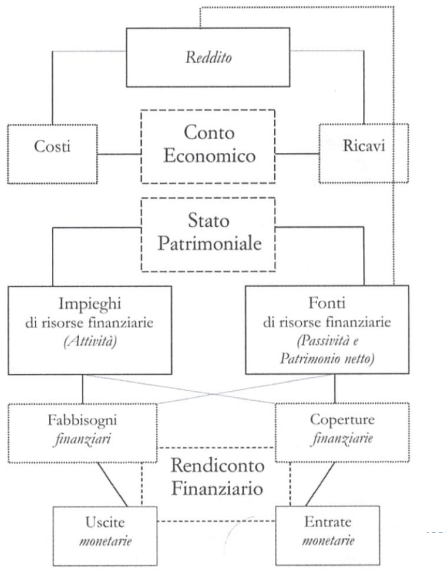
\includegraphics[width=0.4\linewidth]{2/img/Screenshot from 2022-07-09 16-50-17.png}
\end{figure}

\subsection{Classificazione delle voci in base alla determinazione dei valori}
\begin{figure}[H]
    \centering
    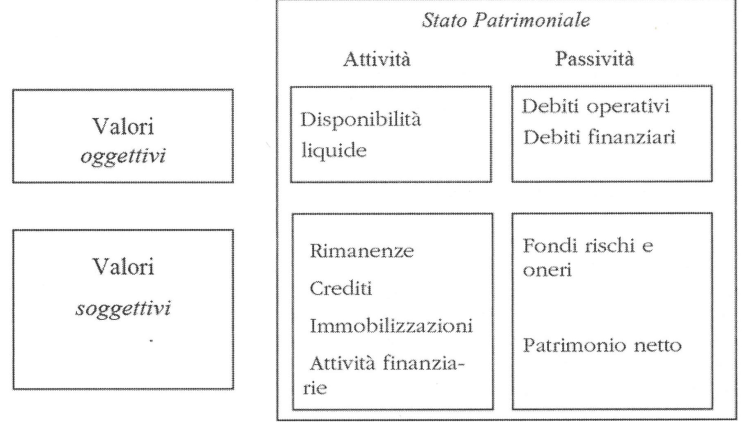
\includegraphics[width=0.4\linewidth]{2/img/Screenshot from 2022-07-09 18-21-32.png}
\end{figure}
\begin{figure}[H]
    \centering
    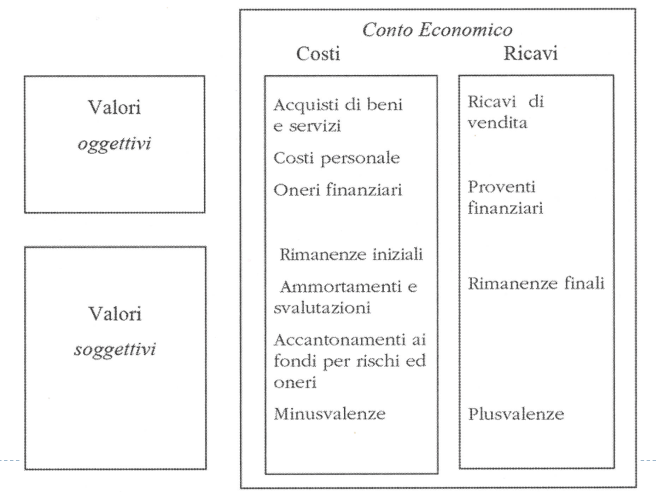
\includegraphics[width=0.4\linewidth]{2/img/Screenshot from 2022-07-09 18-22-41.png}
\end{figure}

\subsection{Analisi del bilancio}
Analizzare i dati contabili ed extra-contabili per valutare e giudicare la gestione aziendale.

Si confrontano i dati di più bilanci per avere una cmparazione temporale(stessa impresa) o comparazione spaziale(differenti aziende).

L'analisi del bilancio è volta a determinare lo stato di salute dell'azienda sulla base
si tre fattori che devono mantersi in equilibrio fra di loro:
\begin{itemize}
    \item economico: produrre reddito per periodo ampio e remunerare i fattori produttivi
    \item patrimoniale: equilibrio tra attività e passività + patrimonio netto
    \item finanziario: rispondere in modo tempestivo agli impegni assunti
\end{itemize}

\subsection{Analisi di bilancio: prospettive}
\begin{figure}[H]
    \centering
    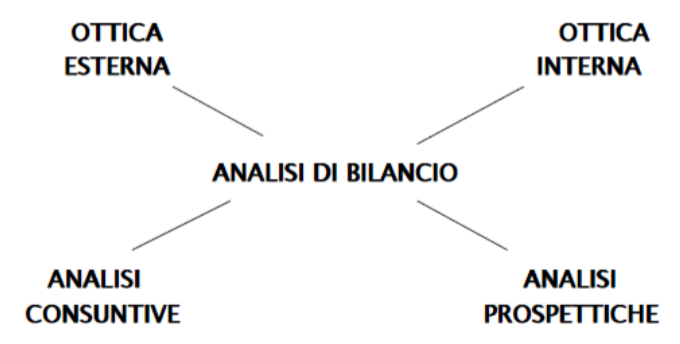
\includegraphics[width=0.5\linewidth]{2/img/Screenshot from 2022-07-10 10-42-56.png}
\end{figure}

\subsubsection{Articolazione}
\begin{figure}[H]
    \centering
    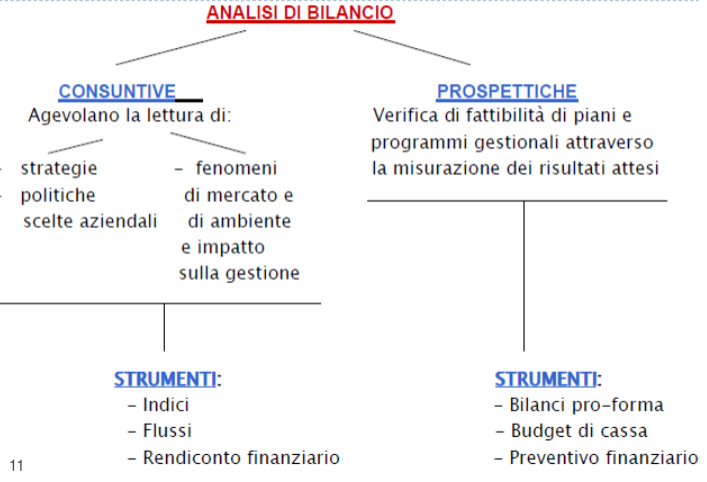
\includegraphics[width=0.5\linewidth]{2/img/Screenshot from 2022-07-10 10-47-54.png}
\end{figure}

\subsubsection{Analisi di bilancio: ottica}
Analisi interne: 
\begin{itemize}
    \item basate sulla documentazione aziendale
    \item completo e tempestivo
    \item riservatezza dei dati permette un bilancio migliore
\end{itemize}


Analisi esterne: 
\begin{itemize}
    \item basato sul bilnacio pubblico
    \item esigenze di riservatezza sull'informazioni(qualità inferiore)
\end{itemize}

\subsubsection{Fasi dell'analisi di bilancio}
\begin{enumerate}
    \item Ricerca ei dati contabili ed extracontabili e loro interpretazioni
    \item riclassificazione dello stato patrimoniale e del conto economico
    \item analisi per indici
    \item analisi per flussi
    \item valutazione dei risultati
\end{enumerate}

Raggruppando le voci di bilancio in gruppi omogenei si facilità il compito di confronto con valori precedenti dei dati e si migliora la lettrua critica.


\subsection{Riclassificazione del conto economico}
Dati aggregati in:
\begin{itemize}
    \item gestione caratteristica(o operativa): costi e ricavi dell'attività di acquisto, trasformazione e vendita
    \item gestione extra-caratteristica(o extra-operativa): 
        \begin{itemize}
            \item gestione accessoria(o straordinaria): attività continuative con con sono l'obiettivo dell'azienda
            \item gestione finanziaria: risultati di operazioni di reperimento di capitale e dell'investimento di risorse liquide
            \item gestione fiscale: elementi di natura fiscale
        \end{itemize}
\end{itemize}

Il principio comune è quello di separare le caratteristiche operative da quelle extra-operative.


Avendo il \textbf{ricavo netto di vendita}, si sottrae il \textbf{costo dei prodotti venduti} e si ottiene 
il \textbf{risultato lordo}.

Poi si sottraggono dal \textbf{risultato lordo} tutte le spese e si ottiene il \textbf{risultato operativo}.

\subsection{Conto Economico a ricavi e costo del
venduto: gestione extra-caratteristica}

\begin{figure}[H]
    \centering
    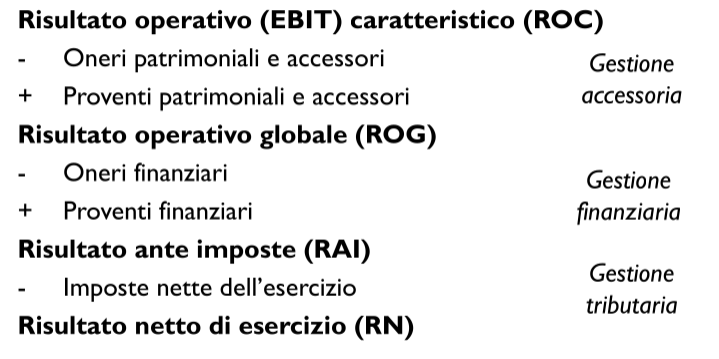
\includegraphics[width=0.5\linewidth]{2/img/Screenshot from 2022-07-10 11-21-34.png}
\end{figure}

\subsection{Conto economico a valore aggiunto}
Ordina i costi per natra economica, la classificaione è in linea con quello civilistica, eichiede meno informazioni rispetto
al conto economico a ricavi e costi del venduto ed è preferito dagli analisti esterni.


\begin{figure}[H]
    \centering
    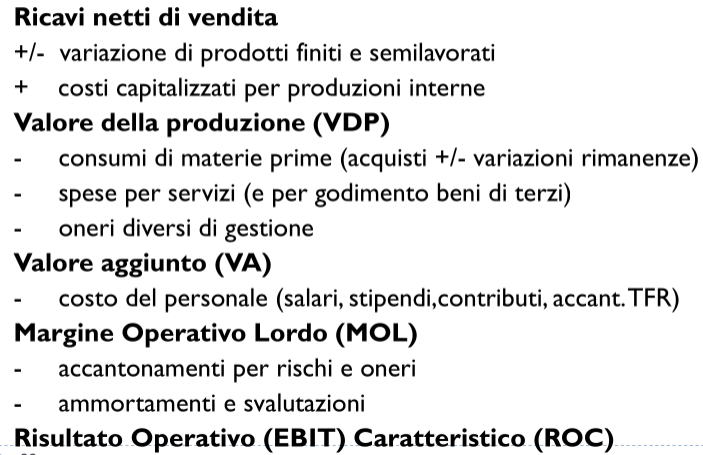
\includegraphics[width=0.5\linewidth]{2/img/Screenshot from 2022-07-10 11-33-38.png}
\end{figure}


\section{Da rifare per bene}